This package provides functions to analyze sets of objects in 2D and 3D. It provides the computation of axis-aligned bounding boxes, centers of mass and principal component analysis for all bounded objects, as well as barycenters for sets of weighted points.\\


\section{Definitions}

A \emph{bounding box} for a set of objects is a cuboid that contains the set. An \emph{axis-aligned bounding box} is a an expression of the maximum extents of all objects from the set within their coordinate system, i.e., a bounding box aligned with the axes of the coordinate system. Axis-aligned bounding boxes are frequently used in geometric algorithms as an indication of the general position of a data set, for either display, first-approximation spatial query, or spatial indexing purposes. \\

A \emph{centroid} of a set of objects is their center of mass, i.e., the point whose coordinates are computed by means of coordinates of all points composing the objects. Note that although the general definition of center of mass incorporates a density function (and hence weighted means), the current implementation assumes a uniform density (see barycenter below defined for weighted points). For a point set $\{X_1,X_2,...,X_N\}$ the centroid $\bar{X}$ is computed as $$\bar{X} = \frac{1}{N} \sum_{i=1}{N} X_i.$$ For a set of segments $\{S_1,S_2,...,S_N\}$ the centroid $\bar{X}$ is computed as $$\bar{X} = \frac{1}{\sum_{i=1}{N}\|S_i\|} \sum_{i=1}{N} \|S_i\|} \bar{S_i},$$ where $\|S_i\|$ stands for the length of a segment and $\bar{S_i}$ stands for its uniform barycenter (midpoint). For a set of triangles $\{T_1,T_2,...,T_N\}$ the centroid $\bar{X}$ is computed as $$\bar{X} = \frac{1}{\sum_{i=1}{N}\|T_i\|} \sum_{i=1}{N} \|T_i\|} \bar{T_i},$$ where $\|T_i\|$ stands for the area of a triangle and $\bar{T_i}$ stands for its uniform barycenter. Such definition still holds for more general objects where the Lebesgue measure (length in 1D, area in 2D, volume in 3D) is used for weighting the object barycenters. Centers of mass are used to summarize data sets for either approximation, spatial query or spatial indexing purposes.\\

A \emph{barycenter} of a set of weighted points is the point whose coordinates are computed by means of weighted coordinates of all weighted points from the set. When all weights are equal the barycenter coincides with the centroid.\\

Given a point set, \emph{linear least squares fitting} amounts to find the linear sub-space which minimizes the sum of squared distances from the points to their projection onto this linear sub-space. 

This problem is equivalent to search for the linear sub-space which maximizes the variance of projected points, the latter being obtained by eigen decomposition of the covariance matrix of the point set. Eigenvectors corresponding to large eigenvalues are the
directions in which the data has strong component, or equivalently large variance. If eigenvalues are the same there is no preferable sub-space.\\

Given an object set, \emph{linear least squares fitting} amounts to find the linear sub-space which minimizes the sum of squared distances from all points in the set to their projection onto this linear sub-space. This problem is equivalent to the one of fitting a linear sub-space to a point set, except that the covariance matrix is now derived (closed form formula) from a continuous integral over the objects instead of a discrete sum over the points.


\begin{center}
    \label{fit}
    % Image
    \begin{ccTexOnly}
      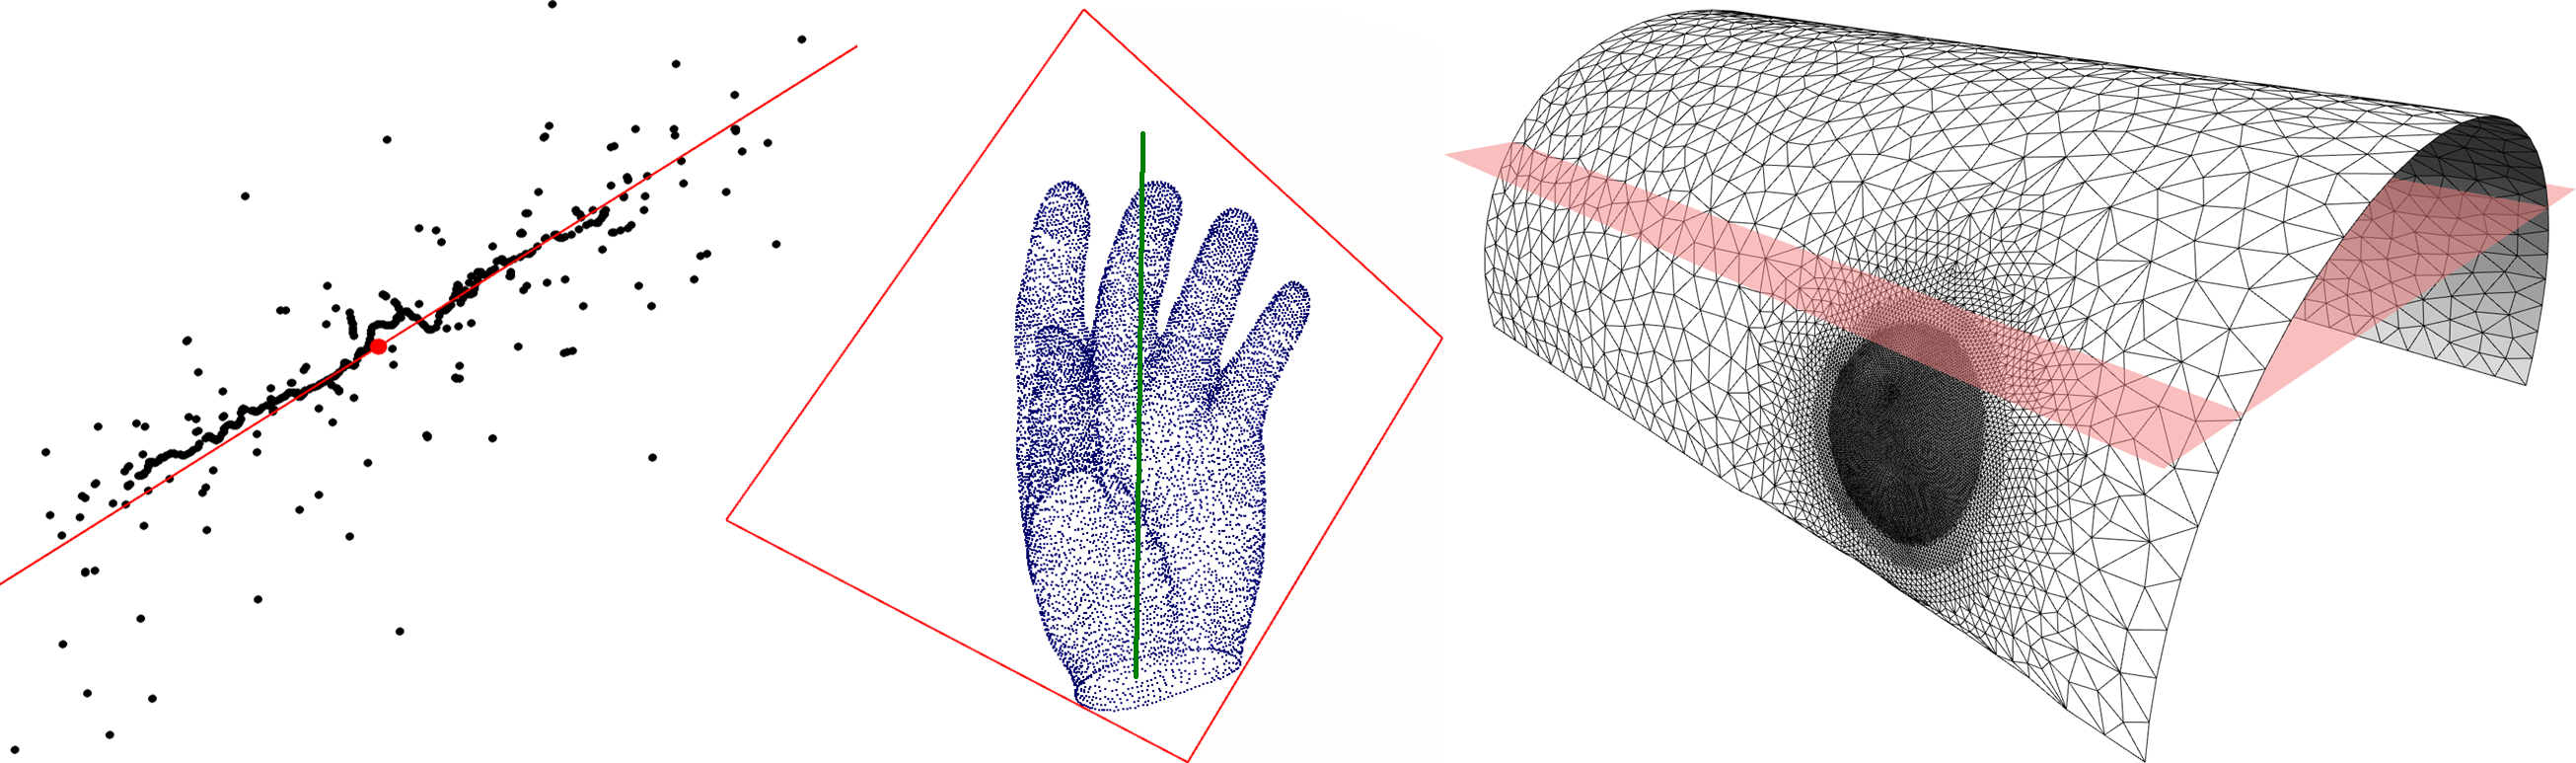
\includegraphics[width=1.0\textwidth]{Principal_component_analysis/fit}
    \end{ccTexOnly}
    \begin{ccHtmlOnly}
        <img width="100%" border=0 src="./fit.png"><P>
    \end{ccHtmlOnly}
    % Title
    \begin{figure}[h]
        \caption{Left: fitting a line to a 2D point set.
                 Right: fitting a line and a plane to a 3D point set.}
    \end{figure}
\end{center}

